\documentclass[16pt, a4paper, two column]{article}
\usepackage[utf8]{inputenc}
\usepackage{mathtools}
\usepackage[a4paper, total={6in, 8in}, margin = 1in]{geometry}
\usepackage{enumitem}
\usepackage{graphicx}
\graphicspath{{images/}}
\usepackage{amsmath}
\newcommand{\myvec}[1]{\ensuremath{\begin{pmatrix}#1\end{pmatrix}}}
\let\vec\mathbf
\title{AI1110 Assignment 1}
\author{Hema Sri Cheekatla, CS21BTECH11013}
\begin{document}
\maketitle
\section*{Question 4a}
Solve the following inequation, write down the solution set and represent it on the real number line:
\begin{align*}
  -2 + 10x \leq 13x + 10 < 24 + 10x,  x\in \mathbb{Z} 
\end{align*}
\section*{Solution}
\begin{align}
  -2 + 10x \leq 13x + 10 < 24 + 10x,  x\in \mathbb{Z} 
\end{align}
\noindent Let us solve the above expression geometrically.

now consider each equation in this expression as a line,i.e., $L_1$ $L_2$ ans $L_3$
\begin{align}
L_1 &\equiv 10x-y-2  \\
L_2 &\equiv 13x-y+10 \\
L_3 &\equiv 10x-y+24
\end{align}
Clearly slopes of $L_1$ and $L_3$ are same i.e., $slope = 10$\newline
and $L_1 \leq L_2 < L_3 $, so the integral values of x on x-axis satisfying this inequality are the required solution set.
In vector form,
\begin{align}
	L_1 &\equiv \myvec{10 & -1}\vec{x} = 2 \\
	L_2 &\equiv \myvec{13 & -1} \vec{x} = -10 \\
	L_3 &\equiv \myvec{10 & -1}\vec{x} = -24
\end{align}
So we need to find the range of x at where the line $L_2$ lies between between line $L_1$ and the line $L_3$

We can obtain the intersection point of $L_1$ and $L_2$ by the following way,
\begin{align}
	\myvec{10 & -1 \\
		13 & -1}\vec{x} &= \myvec{2 \\ -10} 
\end{align}
The augmented matrix for the above matrix equation is 
\begin{align}
	\myvec{ 10 & -1 & \vrule & 2 \\
		13 & -1 & \vrule & -10} \\
	\xleftrightarrow[]{R_2 \leftarrow 10R_2-13R_1}
		\myvec{ 10 & -1 & \vrule & 2 \\
			0 & 3 & \vrule & -126} \\
	\xleftrightarrow[]{R_1 \leftarrow 3R_1+R_2}
		\myvec{ 30 & 0 & \vrule & -120 \\
			0 & 3 &\vrule & -126} \\
	\xleftrightarrow[]{R_1 \leftarrow R_1/30}
		\myvec{ 1 & 0 & \vrule & -4 \\
			0 & 3 & \vrule & -126} \\
	\xleftrightarrow[]{ R_2 \leftarrow R_2/3}
		\myvec{ 1 & 0 & \vrule & -4 \\
			0 & 1 & \vrule & -42} \\
	\implies \vec{x} = \myvec{-4 \\ -42}
\end{align}
Hence the point of intersection of lines $L_1$ and $L_2$ is $\myvec{-4 \\ -42}$ .\newline
Similarly we get the x value at intersection point of lines $L_2$ and $L_3$
\begin{align}
	\myvec{10 & -1 \\
		13 & -1}\vec{x} &= \myvec{-24 \\ -10}
\end{align}
The augmented matrix for the above matrix equation is 
\begin{align}
	\myvec{ 10 & -1 & \vrule & -24 \\
		13 & -1 & \vrule & -10} \\
	\xleftrightarrow[]{R_2 \leftarrow 10R_2-13R_1}
		\myvec{ 10 & -1 & \vrule & -24 \\
			0 & 3 & \vrule & 212} \\
	\xleftrightarrow[]{R_1 \leftarrow 3R_1+R_2}
		\myvec{ 30 & 0 & \vrule & 140 \\
			0 & 3 &\vrule & 212} \\
	\xleftrightarrow[]{R_1 \leftarrow R_1/30}
		\myvec{ 1 & 0 & \vrule &  4.67\\
			0 & 3 & \vrule & 212} \\
	\xleftrightarrow[]{R_2 \leftarrow R_2/3}
		\myvec{ 1 & 0 & \vrule &  4.67\\
			0 & 1 & \vrule & 70.67} \\
	\implies \vec{x} = \myvec{4.67 \\ 70.67}
\end{align}
Hence the point of intersection of lines $L_2$ and $L_3$ is $\myvec{4.67 \\ 70.67}$.\newline
%\vspace{16pt}

Since $L_1 \leq L_2 < L_3$, this implies the corresponding x-coordinates follows, $-4 \leq x < 4.67$ \newline

\noindent Now let us draw the corresponding lines

\begin{figure}[h]
  %  \centering
    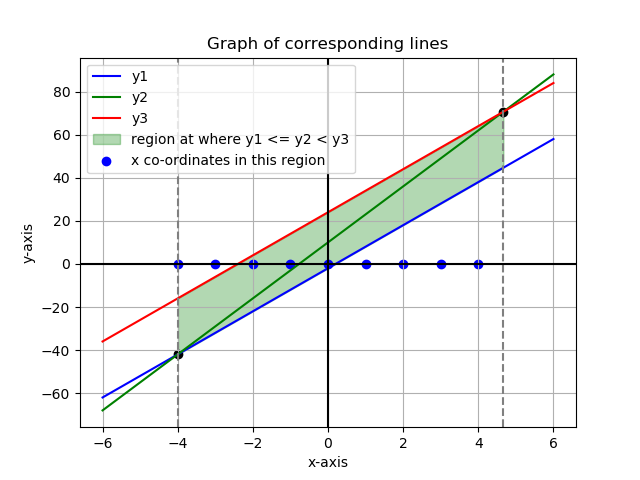
\includegraphics[width = \columnwidth]{Figure_1}
    \caption{lines $L_1$, $L_2$ and $L_3$}
    \label{fig:mesh1}
\end{figure}

%\vspace{16pt}

\noindent If we observe this graph, it is clear that the lines $L_1$ and $L_2$ are intersecting at $x = -4$ and the lines $L_2$ and $L_3$ are intersecting at some point where $x>4$ \newline
%\vspace{10pt}

Hence the required range of x is $[\ -4, 4.67)\ $\newline


%\vspace{10pt}
\noindent Therefore the integers in this range are,

\begin{center}
\begin{tabular}{|c|}
\hline
\textbf{$ \{ -4, -3, -2, -1, 0, 1, 2, 3, 4\}$} \\
\hline
\end{tabular}
\end{center}


\noindent Here is the plot of corresponding points on the real number line\\
\begin{figure}[h]
   % \centering
    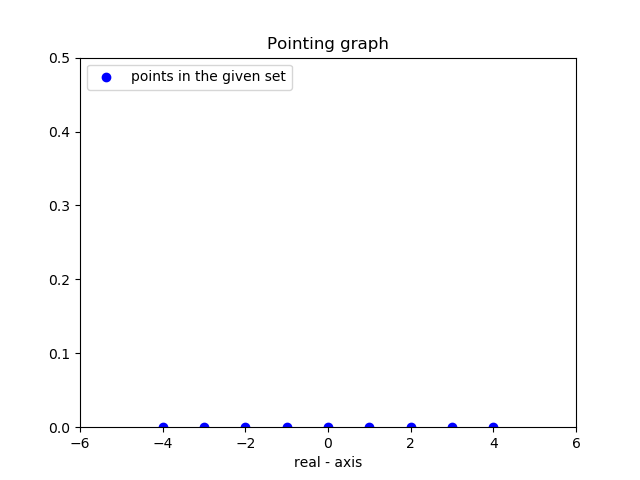
\includegraphics[width =\columnwidth]{Figure_2}
    \caption{set of points that obey given expression on real number line}
    \label{fig:mesh1}
\end{figure}
\end{document}
